\input{./econtexRoot.texinput}
\documentclass[\econtexRoot/HAFiscal]{subfiles}

% \onlyinsubfile{\renewcommand{\econtexRoot}{..}} % 
\onlyinsubfile{\externaldocument{\econtexRoot/HAFiscal}} % Get xrefs -- esp to apndx -- from main file; only works if main file
\begin{document}

\section{Parameterizing the model}

This section describes how we set the model's parameters. First, we estimate the extent to which consumers `splurge' when receiving an income shock. We do so using Norwegian data to allow the model to match the best available evidence on the time profile of the marginal propensity to spend provided by \citet{fagereng_mpc_2021}. For this exercise, we use a version of the model calibrated to the Norwegian economy. 

Second, we calibrate the full model on U.S. data, taking the splurge factor as given from the Norwegian calibration. In the model, agents differ according to their level of education and their subjective discount factors. %Some parameters are calibrated equally for all of these different types, while some are calibrated separately for each education group.
Finally, a distribution of subjective discount factors is estimated separately for each education group to match features of each within-group liquid wealth distribution. 

\subsection{Estimation of the splurge factor}
\notinsubfile{\label{sec:splurge}}

We define splurging as the free spending of current labor income without concern for intertemporal maximization of utility. The splurge allows us to capture the shorter- and longer-term response of consumption to income shocks, especially for consumers with significant liquid wealth, that a standard model cannot. Specifically, we show that our model can account well for the results of \citet{fagereng_mpc_2021}, who study the effect of lottery winnings in Norway on consumption using millions of records from the Norwegian population registry. Using their results, we calibrate our model to reflect the Norwegian economy and estimate the splurge factor, as well as the distribution of discount factors in the population, to match two empirical moments. 

First, we take from \citet{fagereng_mpc_2021} the marginal propensity to consume out of a one-period income shock. We target not only the initial response of consumption to the income shock, but also the subsequent effect on consumption in years one through four after the shock. The shares of lottery winnings expended at different time horizons, as found in \citet{fagereng_mpc_2021}, are plotted in figure \ref{fig:aggmpclotterywin}. Note that the first-year expenditure, shown in figure \ref{fig:aggmpclotterywin} to be around 0.5, is not equivalent to the initial annual MPC because the lottery winnings may occur toward the end of the year. %\citet{fagereng_mpc_2021} estimate that their suggests an initial annual MPC of 0.63.

Second, we match the steady-state distribution of liquid wealth in the model to its empirical counterpart. Because of the lack of data on the liquid wealth distribution in Norway, we use the corresponding data from the United States---assuming that liquid wealth inequality is comparable across these countries.\footnote{Data from the Norwegian tax registry contains information on liquid assets, but not liquid debt. Only total debt is reported -- which is mainly mortgage debt. Therefore, we cannot construct liquid wealth as \citet{kaplan2014model} can for the U.S. \notinsubfile{\label{foot:liqwealth}} Specifically, we impose as targets the cumulative liquid wealth shares for the entire population at the 20th, 40th, 60th, and 80th income percentiles, which, in data from the Survey of Consumer Finances (SCF) in 2004, equal $0.03$ percent, $0.35$ percent, $1.84$ percent, and $7.42$ percent, respectively.\footnote{See section~\ref{sec:SCFdata} for details.} Hence, $92.6$ percent of the total liquid wealth is held by the top income quintile. The data are plotted in figure \ref{fig:liquwealthdistribution}}.

\begin{figure}[htb]
  \centering
  \begin{subfigure}[b]{.48\linewidth}
    \centering
    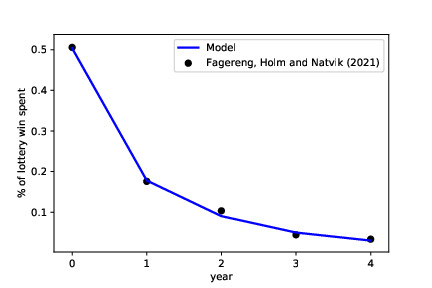
\includegraphics[width=\linewidth]{\econtexRoot/Code/HA-Models/Target_AggMPCX_LiquWealth/Figures/AggMPC_LotteryWin}
    \caption{Share of lottery win spent}
    \notinsubfile{\label{fig:aggmpclotterywin}}
  \end{subfigure}
  \begin{subfigure}[b]{.48\linewidth}
    \centering
    
\includegraphics[width=\linewidth]{\econtexRoot/Code/HA-Models/Target_AggMPCX_LiquWealth/Figures/LiquWealth_Distribution}
    \caption{Distribution of liquid wealth}
    \notinsubfile{\label{fig:liquwealthdistribution}}
  \end{subfigure}%
  \caption{Targets and model moments from the estimation}
  \notinsubfile{\label{fig:splurge_estimation}}
  \parbox{16cm}{\small \vspace{.15cm} \textbf{Note}: Panel (a) shows the fit of the model to the dynamic consumption response estimated in \citet{fagereng_mpc_2021}; see their figure~A5. Panel (b) shows the fit of the model to the distribution of liquid wealth (see Section~\ref{sec:SCFdata} for the definition) from the 2004 SCF.\normalsize}
\end{figure}


For this estimation exercise, the remaining model parameters are calibrated to reflect the Norwegian economy. Specifically, we set the real interest rate to $2$ percent annually and the unemployment rate to $4.4$ percent, in line with \citet{aursland_state-dependent_2020}. The quarterly probability to survive is calibrated to $1-1/160$, reflecting an expected working life of 40 years. Aggregate productivity growth is set to $1$ percent annually, following \citet{kravik_navigating_2019}. The unemployment net replacement rate is calibrated to $60$ percent, following \citet{oecd_net_2020}. Finally, we set the real interest rate on liquid debt to $13.6$ percent and the borrowing constraint to $80$ percent of permanent income, following data from the Norwegian debt registry \citet{gjeldsregistret_nokkeltall_2022}.\footnote{Specifically, we determine the average volume-weighted interest rate on liquid debt, which consists of consumer loans, credit and payment card debt and all other unsecured debt. To determine the borrowing limit on liquid debt we calculate the ratio of the total credit card limit to total wage income in Norway. We use data from December 2019. Note that although these data let us pin down aggregate quantities, they do not solve the issue referred to in footnote~\ref{foot:liqwealth}, since we cannot link them to the tax registry at the individual level.}

Estimates of the standard deviations of the permanent and transitory shocks are taken from \citet{crawley2022parsimonious}, who estimate an income process on administrative data for Norwegian males from 1971 to 2014. The estimated annual variances for the permanent and transitory shocks are 0.004 and 0.033, respectively.\footnote{As shown in \citet{crawley2022parsimonious}, an income process of the form that we use here is more accurately estimated using moments in levels not differences. Hence, we take the numbers from column 3 of their table 4.} As in \citet{carroll2020sticky}, these are converted to quarterly values by multiplying the permanent and transitory shock variances by $1/4$ and $4$, respectively. Thus, we obtain quarterly standard deviations of $\sigma_\psi=0.0316$ and $\sigma_\xi=0.363$.

Using the calibrated model, we simulated unexpected lottery winnings and calculate the share of the lottery spent in each year. Specifically, each simulated agent receives a lottery win in a random quarter of the first year of the simulation. The size of the lottery win is itself random and spans the range of lottery sizes found in \citet{fagereng_mpc_2021}. The estimation procedure minimizes the distance between the target and model moments by selecting the splurge factor and the distribution of discount factors in the population, where the latter are assumed to be uniformly distributed in the range $[\beta-\nabla, \beta+\nabla]$. We approximate the uniform distribution of discount factors with a discrete approximation and let the population consist of seven different types.

The estimation yields a splurge factor of $0.314$ and a distribution of discount factors described by $\beta = 0.989$ and $\nabla=0.0179$. Given these estimated parameters and the remaining calibrated ones, the model is able to replicate the time path of consumption in response to a lottery win from \citet{fagereng_mpc_2021} and the targeted distribution of liquid wealth very well (see figure \ref{fig:splurge_estimation}).


\subsection{Data on permanent income, liquid wealth, and education}
\notinsubfile{\label{sec:SCFdata}}

Before we move on to the parameterization of the full model, we describe in detail the data that we use to get measures of permanent income, liquid wealth, and the division of households into educational groups in the United States. We use data on the distribution of liquid wealth from the 2004 wave of the SCF. We restrict our attention to households where the head is of working age, which we define to be in the range from 25 to 62. The SCF-variable ``normal annual income'' is our measure of the household's permanent income, and, to exclude outliers, we drop the observations that make up the bottom 5 percent of the distribution of this variable. The smallest value of permanent income for households in our sample is thus \$16,708. 

Liquid wealth is defined as in \cite{kaplan2014model} and consists of cash, money market, checking, savings, and call accounts; directly held mutual funds; and stocks and bonds. We subtract off liquid debt, which is the revolving debt on credit card balances. Note that the SCF does not contain information on cash holdings, so these are imputed with the procedure described in Appendix B.1 of \cite{kaplan2014model}, which also describes the credit card balances that are considered part of liquid debt. We drop any households that have negative liquid wealth. 

Households are classified into three educational groups. The first group, ``Dropout,'' applies to households where the head of household has not obtained a high school diploma; the second group, ``Highschool,'' includes heads of households who have a high school diploma and those who, in addition, have some years of college education without obtaining a bachelor's degree; and the third group, ``College,'' consists of heads of households who have obtained a bachelor's degree or higher. With this classification of the education groups, the Dropout group makes up $9.3$ percent of the population, the Highschool group $52.7$ percent, and the College group $38.0$ percent. 

With our sample selection criteria, we are left with a sample representing about 61.3 million U.S. households.

\subsection{Calibrated parameters} 
\notinsubfile{\label{sec:calib}}

With households divided into the three education groups, some parameters, presented in panel~A of table~\ref{tab:calibration}, are calibrated equally across all groups, while other parameters, presented in panel~B of table~\ref{tab:calibration}, are education specific.  Households are also assumed to be ex-ante heterogeneous in their subjective discount factors as well as their level of education. For completeness, panel~C of table~\ref{tab:calibration} summarizes the parameters describing how we model a recession and the three policies we consider as potential responses to a recession. 

All households are assumed to have a coefficient of relative risk aversion equal to $\gamma=2$. We also assume that all households have the same propensity to splurge out of transitory income gains and set $\varsigma=0.314$, the value estimated in section~\ref{sec:splurge}. However, each education group is divided into types that differ in their subjective discount factors. The distributions of discount factors for each education group are estimated to fit the distribution of liquid wealth within that group, and this estimation is described in detail in section~\ref{sec:estimBetas}. Regardless of type, households face a constant survival probability each quarter. This probability is set to $1-1/160$, reflecting an expected working life of 40 years. The real interest rate on households' savings is set to $1$ percent per quarter. 

\afterpage{
  \thispagestyle{empty}
  \begin{table}[p]
    \begin{center}
      \begin{tabular}{l}
        \begin{tabular}{lcd{3}} 
          \toprule
          \multicolumn{3}{l}{Panel (A) Parameters that apply to all types} \\ \midrule
          Parameter & Notation & \text{Value} \\ \midrule 
          Risk aversion & $\gamma$ & 2.0 \\ 
          Splurge & $\varsigma$ & 0.307 \\ 
          Survival probability, quarterly & $1-D$ & 0.994 \\
          Risk free interest rate, quarterly (gross) & $R$ & 1.01 \\ 
          Standard deviation of transitory shock & $\sigma_\xi$ & 0.346 \\
          Standard deviation of permanent shock & $\sigma_\psi$ & 0.0548 \\ 
          Unemployment benefits replacement rate (share of PI) & $\rho_b$ & 0.7 \\ 
          Unemployment income w/o benefits (share of PI) & $\rho_{nb}$ & 0.5 \\ 
          Avg. duration of unemp. benefits in normal times (quarters) & & 2 \\
          Avg. duration of unemp. spell in normal times (quarters) & & 1.5 \\
          Probability of leaving unemployment & $\pi_{ue}$ & 0.667 \\ 
          Consumption elasticity of aggregate demand effect & $\kappa$ & 0.3 
          \\ \bottomrule 
        \end{tabular} \\ \\

        \begin{tabular}{lccc}
          \toprule 
          \multicolumn{4}{l}{Panel (B) Parameters calibrated for each education group} \\ \midrule
          & Dropout & Highschool & College \\ \midrule
          Percent of population & \phantom{0}9.3 & 52.7 & 38.0 \\ 
          Avg. quarterly PI of ``newborn'' agent (\$1000) & \phantom{0}6.2 & 11.1 & 14.5 \\
          Std. dev. of $\log($PI$)$ of ``newborn'' agent & 0.32 & 0.42 & 0.53 \\
          Avg. quarterly gross growth rate of PI ($\Gamma_e$) & 1.0036 & 1.0045 & 1.0049 \\
          Unemployment rate in normal times (percent) & \phantom{0}8.5 & \phantom{0}4.4 & \phantom{0}2.7 \\ 
          Probability of entering unemployment ($\pi_{eu}^{e}$, percent) & \phantom{0}6.2 & \phantom{0}3.1 & \phantom{0}1.8 
          \\ \bottomrule 
        \end{tabular} \\
        \parbox{16cm}{\small \vspace{.25cm} \textbf{Note}: The first three rows show numbers from the 2004 SCF. The fourth row are averages of growth rates from \cite{carroll2020modeling}. The fifth row are numbers for 2004 from statista.com, and the sixth row are calculated from these unemployment rates.\normalsize}
        \\ \\

        \begin{tabular}{lc}
          \toprule 
          \multicolumn{2}{l}{Panel (C) Parameters describing policy experiments} \\ \midrule 
          Parameter & Value \\ \midrule 
          Change in unemployment rates in a recession & $\times 2$ \\ 
          Expected unemployment spell in a recession & 4 quarters \\ 
          Average length of recession & 6 quarters \\ 
          Size of stimulus check & \$1,200 \\ 
          PI threshold for reducing check size & \$100,000 \\ 
          PI threshold for not receiving check & \$150,000 \\ 
          Extended unemployment benefits & 4 quarters \\
          Length of payroll tax cut & 8 quarters \\ 
          Income increase from payroll tax cut & 2 percent \\ 
          Belief (probability) that tax cut is extended & 50 percent 		
          \\ \bottomrule
        \end{tabular} 

      \end{tabular}
    \end{center}
    \caption{Panel (A) shows parameters calibrated the same for all types. Panel (B) shows parameters calibrated for each education group. Panel (C) shows the numbers describing how we model a recession and the three policies we consider. ``PI'' refers to permanent income.}
    \notinsubfile{\label{tab:calibration}}
  \end{table}
  \clearpage
}

% \begin{table}[th]
%   \begin{center}
%     \begin{tabular}{lcd{3}} 
        %         \toprule
        %         Parameter & Notation & $\text{Value}$ \\ \midrule 
        %         Risk aversion & $\gamma$ & 1.0 \\ 
        %         Splurge & $\varsigma$ & 0.32 \\ 
        %         Survival probability, quarterly & $1-D$ & 0.994 \\
        %         Risk free interest rate, quarterly (gross) & $R$ & 1.01 \\ 
        %         Standard deviation of transitory shock & $\sigma_\xi$ & 0.346 \\
        %         Standard deviation of permanent shock & $\sigma_\psi$ & 0.0548 \\ 
        %         Unemployment benefits replacement rate (share of PI) & $\rho_b$ & 0.3 \\ 
        %         Unemployment income w/o benefits (share of PI) & $\rho_{nb}$ & 0.05 \\ 
        %         Avg. duration of unemp. spell in normal times (quarters) & & 1.5 \\
        %         Avg. duration of unemp. benefits in normal times (quarters) & & 2 
                                                                                  %         \\ \bottomrule 
        %       \end{tabular}
        %         \caption{Calibrated parameters that apply to all types. ``PI'' refers to permanent income.}
        %         \notinsubfile{\label{tab:calibAll}}
        %         \end{center}	
        %         \end{table}

When consumers are born, they receive an initial level of permanent income. This initial value is drawn from a log-normal distribution that depends on the education level the household is born with. For each education group, the parameters of the distribution are determined by the mean and standard deviation of log-permanent income for households of age 25 in that education group in the SCF 2004. For the Dropout group, the mean initial value of quarterly permanent income is \$6,200; for the Highschool group, it is \$11,100; and for the College group, it is \$14,500. The standard deviations of the log-normal distributions for each group are, respectively, $0.32$, $0.42$, and $0.53$. 

        %         \begin{table}[th]
        %         \begin{center}
        %         \begin{tabular}{lccc}
        %         \toprule 
        %         \multicolumn{4}{l}{Parameters calibrated for each education group} \\ 
        %                             & Dropout & Highschool & College \\ \midrule
        %         Percent of population & \phantom{0}9.3 & 52.7 & 38.0 \\ 
        %         Avg. quarterly PI of ``newborn'' agent (\$1000) & \phantom{0}6.2 & 11.1 & 14.5 \\
        %         Std. dev. of $\log($PI$)$ of ``newborn'' agent & 0.32 & 0.42 & 0.53 \\
        %         Avg. quarterly gross growth rate of PI & 1.0036 & 1.0045 & 1.0049 \\
        %         Unemployment rate in normal times (percent) & \phantom{0}8.5 & \phantom{0}4.4 & \phantom{0}2.7  			
                                                                                                  %         \\ \bottomrule 
        %       \end{tabular}
        %         \caption{Parameters calibrated for each education group. ``PI'' refers to permanent income.}
        %         \notinsubfile{\label{tab:calibEd}}
        %         \end{center}
        %         \end{table}

While households remain employed, their income is subject to both permanent and transitory idiosyncratic shocks. These shocks are distributed equally for the three education groups. The standard deviations of these shocks are taken from \cite{carroll2020sticky}, who set the standard deviations of the transitory and permanent shocks to $\sigma_\xi=0.346$ and $\sigma_\psi=0.0548$, respectively. Permanent income also grows, on average, with a growth rate $\Gamma_{e(i)}$ that depends on the level of education. These average growth rates are based on numbers from \cite{carroll2020modeling}, who construct age-dependent expected permanent income growth factors using numbers from \cite{cagetti2003wealth} and fit the age-dependent numbers to their life-cycle model. We construct the quarterly growth rates of permanent income in our perpetual-youth model by taking the average of the age-dependent growth rates during a household's working life. The average gross quarterly growth rates that we obtain for the three education groups are then $\Gamma_d=1.0036$, $\Gamma_h=1.0045$, and $\Gamma_c=1.0049$.

Consumers also face the risk of becoming unemployed and will then have access to unemployment benefits for a certain period. The parameters describing the unemployment benefits in normal times are based on the work of \cite{rothstein2017scraping}, who study the effects on household income of unemployment and of running out of eligibility for benefits. The unemployment benefits replacement rate is thus set to $\rho_b=0.7$ for all households, and when benefits run out, the unemployment replacement rate without any benefits is set to $\rho_{nb}=0.5$. These replacement rates are set as a share of the households' permanent income and are based on the initial drop in income upon entering an unemployment spell, presented in figure~3 in \cite{rothstein2017scraping}.\footnote{See the lines for their UI exhaustee sample including and excluding UI income. \cite{rothstein2017scraping} also point out that ``UI benefits replace about 40 percent of the lost earnings on average'' (page 894). For a household with two income earners with equal income, these findings would mean that income drops to 70 percent when one earner becomes unemployed and to 50 percent when benefits run out. In this paper we ignore several of the channels studied by \cite{rothstein2017scraping} such as within household insurance and other social programs that can provide income even after UI benefits have run out.} The duration of unemployment benefits in normal times is set to two quarters, so that our Markov transition matrix $\Pi$ has four states. This length of time corresponds to the mean duration of unemployment benefits across U.S. states from 2004 to mid-2008 of 26 weeks, reported by \cite{rothstein2017scraping}. 

The probability of transitioning out of unemployment is the same for all households and is set to $\pi_{ue}=2/3$. This probability implies that the average duration of an unemployment spell in normal times is one and a half quarters, which is also the value used in \cite{carroll2020modeling}. However, the different education groups do differ in the probability of transitioning into unemployment in the first place. These probabilities are set to match the average U.S. unemployment rate by education group in 2004.\footnote{Source: Statista.com.} This average was 8.5 percent for the Dropout group, 4.4 percent for the Highschool group, and 2.7 percent for the College group. These values imply that the probabilities of transitioning into unemployment in normal times are $\pi_{eu}^d=6.2$ percent, $\pi_{eu}^h=3.1$ percent, and $\pi_{eu}^c=1.8$ percent, respectively. 

Finally, the strength of the aggregate demand effect in recessions is determined by the consumption elasticity of productivity. We follow \cite{kmpHandbook2016} and set this to $\kappa=0.3$. 


\subsection{Estimating the discount factor distributions} 
\notinsubfile{\label{sec:estimBetas}}

Discount factor distributions are estimated separately for each education group to match the distribution of liquid wealth for households in that group. To do so, we let each education group consist of types that differ in their subjective discount factor,~$\beta$. The discount factors within each group $e\in \{d, h, c\}$ are assumed to be uniformly distributed in the range $[\beta_e-\nabla_e, \beta_e+\nabla_e]$. The parameters $\beta_e$ and $\nabla_e$ are chosen for each group separately to match the median liquid-wealth-to-permanent-income ratio and the $\nth{20}$, $\nth{40}$, $\nth{60}$, and $\nth{80}$ percentile points of the Lorenz curve for liquid wealth for that group. We approximate the uniform distribution of discount factors with a discrete approximation and let each education group consist of seven different types.

Panel~A of table~\ref{tab:estimBetas} shows the estimated values of $(\beta_e, \nabla_e)$ for each education group. The panel also shows the minimum and maximum values of the discount factors we actually use in the model when we use a discrete approximation with seven values to approximate the uniform distribution of discount factors. Panel~B of table~\ref{tab:estimBetas} shows that with these estimated distributions, we can exactly match the median liquid-wealth-to-permanent-income ratios for each education group. Figure~\ref{fig:LorenzPts} shows that with the estimated distributions, the model quite closely matches the distribution of liquid wealth within each education group as well as for the population as a whole. Our model does not suffer from the ``missing middle'' problem, identified in \cite{kaplanMPC2022}, in which the middle of the wealth distribution has too little wealth.  Our model avoids this problem for two reasons: (1) The splurge pushes up MPCs relative to wealth, and (2) we calibrate to liquid wealth rather than total wealth.

\begin{table}[tp]
  \begin{center}
    \begin{tabular}{l}
      \begin{tabular}{lccc}
        \multicolumn{4}{l}{Panel (A) Estimated discount factor distributions} \\ 
        & Dropout & Highschool & College \\ \midrule
        $(\beta_e, \nabla_e)$ & (0.694, 0.542) & (0.904, 0.099) & (0.978,0.015) \\
        (Min, max) in approximation & (0.230, 0.995) & (0.819, 0.989) & (0.965, 0.991) \\
        \midrule 
      \end{tabular} \\ \\ 
      
      \begin{tabular}{lccc}
        \multicolumn{4}{l}{Panel (B) Estimation targets} \\ \midrule
        & Dropout & Highschool & College \\ \midrule
        Median LW/ quarterly PI (data, percent) & 4.64 & 30.2 & 112.8 \\ 
        Median LW/ quarterly PI (model, percent) & 4.64 & 30.2 & 112.8 %\\
        %         $[20,40,60,80]$ pctiles of Lorenz curve (data) & $[0, 0.01, 0.6, 3.6]$ & $[0.06, 0.6, 3.0, 11.6]$ & $[0.2, 0.9, 3.3, 10.3]$ \\
        %         $[20,40,60,80]$ pctiles of Lorenz curve (model) & $[0.0, 0.0, 0.5, 3.6]$ & $[0.04, 0.9, 3.7, 11.3]$ & $[0.3, 1.5, 4.0, \phantom{0}9.9]$
        \\ \midrule 
      \end{tabular} \\ \\ 
      
      \begin{tabular}{lcccc}
        \multicolumn{5}{l}{Panel (C) Non-targeted moments} \\ 
        & Dropout & Highschool & College & Population \\ \midrule
        Percent of total wealth (data) & 0.8 & 17.9 & 81.2 & 100 \\
        Percent of total wealth (model) & 12.4 & 18.6 & 69.0 & 100 \\
        Avg. annual MPC (model, incl. splurge) & 0.79 & 0.78 & 0.54 & 0.69
        \\ \bottomrule 
      \end{tabular}
    \end{tabular}
    \caption{Estimated discount factor distributions, estimation targets, and non-targeted moments}
    \notinsubfile{\label{tab:estimBetas}}
    \parbox{16cm}{\small \vspace{.15cm} \textbf{Note}: Panel (A) shows the estimated parameters of the discount distributions for each education group. It also shows the minimum and maximum values we use in our discrete approximation to the uniform distribution of discount factors for each group. Panel (B) shows the weighted median ratio of liquid wealth to permanent income from the 2004 SCF and in the model. In the annual data from the SCF, the annual PI is divided by 4 to obtain a quarterly number. Panel (C) shows percent of total wealth held by each education group in the 2004 SCF and in the model. It also shows the average annual MPCs calculated for each individual from the splurge and the quarterly MPCs, and then averaged by education group.\normalsize}
  \end{center}
\end{table}

There are a few points to note regarding the estimated discount factor distribution for the Dropout group, however. Panel~B of table~\ref{tab:estimBetas} reports that the median liquid-wealth-to-permanent-income ratio for this group is quite low at $4.64$, and the top-left quadrant of figure~\ref{fig:LorenzPts} shows that liquid wealth is very concentrated within this education group, as the bottom 80 percent  hold oly $3.6$ percent of the wealth within the Dropout group. Hence, the estimated discount factor distribution is centered at a very low value, with $\beta_d=0.694$, to get little saving in this group, on average, and the distribution is very wide, with $\nabla_d=0.542$, to get a distribution where wealth is very concentrated. 

\begin{figure}[th]
  \begin{center}
    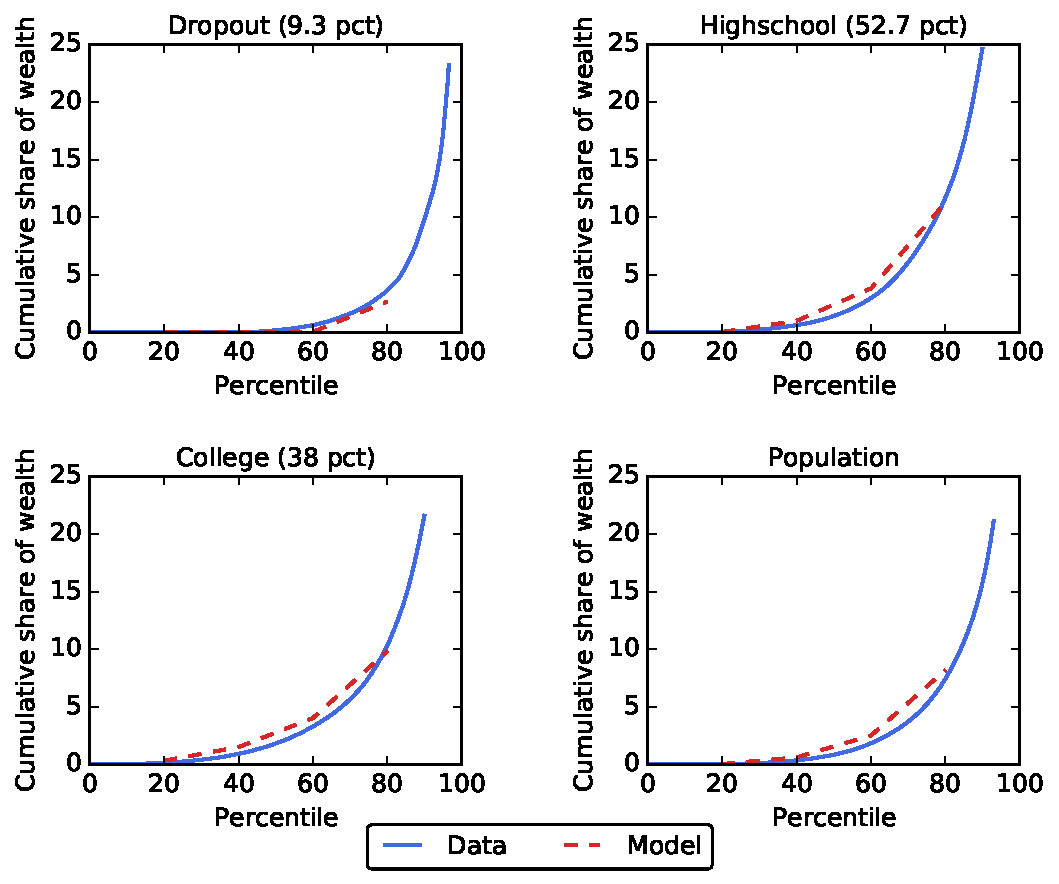
\includegraphics[width=.9\textwidth]{../Figures/LorenzPoints.pdf}
    \caption{Distributions of liquid wealth within each educational group and for the whole population from the 2004 Survey of Consumer Finances and from the estimated model}
    \notinsubfile{\label{fig:LorenzPts}}
  \end{center}
\end{figure}

At the upper end of the discount factor distribution for the Dropout group, these estimates would imply a discount factor far above $1$. However, this value is not actually the relevant constraint on the maximum discount factors. Instead, the maximum value reported in panel~A of table~\ref{tab:estimBetas} is imposed to ensure that the Growth Impatience Condition (GIC), discussed in \cite{carroll2022theoretical}, is always satisfied. This constraint is imposed in the estimation for each education group, but it is binding only for the Dropout group. Thus, the estimation can select a large value of $\nabla_d$ without violating the constraint.\footnote{The constraint is imposed by calculating a value of $\beta$ where the GIC holds with equality and setting the upper bound for admissible discount factors to $0.9975\times$ that value.}

The result is that several of the types in the Dropout group have very low discount factors and are very impatient. In this way, the model fits the feature of the data for the Dropout group that the bottom quintiles do not save at all and do not accumulate any liquid wealth. Very low estimates for discount factors are in line with those obtained in the literature on payday lending.\footnote{See, for example, \cite{skiba2008payday}, who estimate two-week discount rates of $21$ percent, and \cite{allcott2021high}, who estimate an initial period discount factor between $0.74$ and $0.83$ in a model where a period is eight weeks long. Both of these papers use quasi-hyperbolic preferences, so the estimates are not directly comparable with parameters in our model. Nevertheless, they support the point that very high discount rates are necessary to model the part of the population that takes out payday loans at very high interest rates.} 

Finally, panel~C of table~\ref{tab:estimBetas} shows the wealth distribution across the three education groups in the data and in the model. The most patient types in the Dropout group that have discount factors imposed by the GIC constraint accumulate a larger share of wealth in the model than they do in the data. Thus, the model overestimates the share of wealth of the Dropout group as a whole in order to produce a liquid wealth distribution within that group that matches the data. The panel also reports the average marginal propensity to consume within a year after an income shock for each education group. This measure of the annual MPC takes into account the initial splurge factor when an income shock is first received, as well as the decisions to consume out of additional income over four quarters after the shock. The average annual MPC for the population as a whole is $0.69$ in the model, which is slightly higher than the $0.63$ estimated for Norway by \cite{fagereng_mpc_2021}. 

\ifthenelse{\boolean{Web}}{}{
  \end{document} \endinput
}
